\chapter{Signal Processing}\label{ch:signalProcessing}
A sound wave at its most basic form is described as a vibration that propagates in a medium as gas, 
liquid or solid as an audible fluctuation in pressure. A transducer, as a microphone has a diaphragm 
that vibrates according to those fluctuations. In this way the amplitude, the power of pressure, 
can be recorded. Another property of of sound wave is the frequency, which is the variation of 
the amplitude over time, which can be easily calculated from a two dimensional plot, with the 
two axis being the amplitude and the time, looking at the number of occurrences of a cycle in a unit of time.\cite{SOUNDWAVE}

\section{Signal Preprocessing}
As sound is an analog signal, for recording that signal it will have to be sampled. Depending on the 
sampling rate, the sound signal can have varying degree of quality, human ears are most the most 
sensitive in the range of 100 to 3000 Hz which are also called the fundamental frequencies. But 
human voice also has harmonics which are in the range of 900 Hz to 17 KHz.
According to the Nyquist rate of signal processing, the sample rate should be at 
least double the frequency of the signal in order to avoid aliasing.\cite{VOICEFREQUENCY}
\newpage
\begin{figure}[htp]
	\centering
	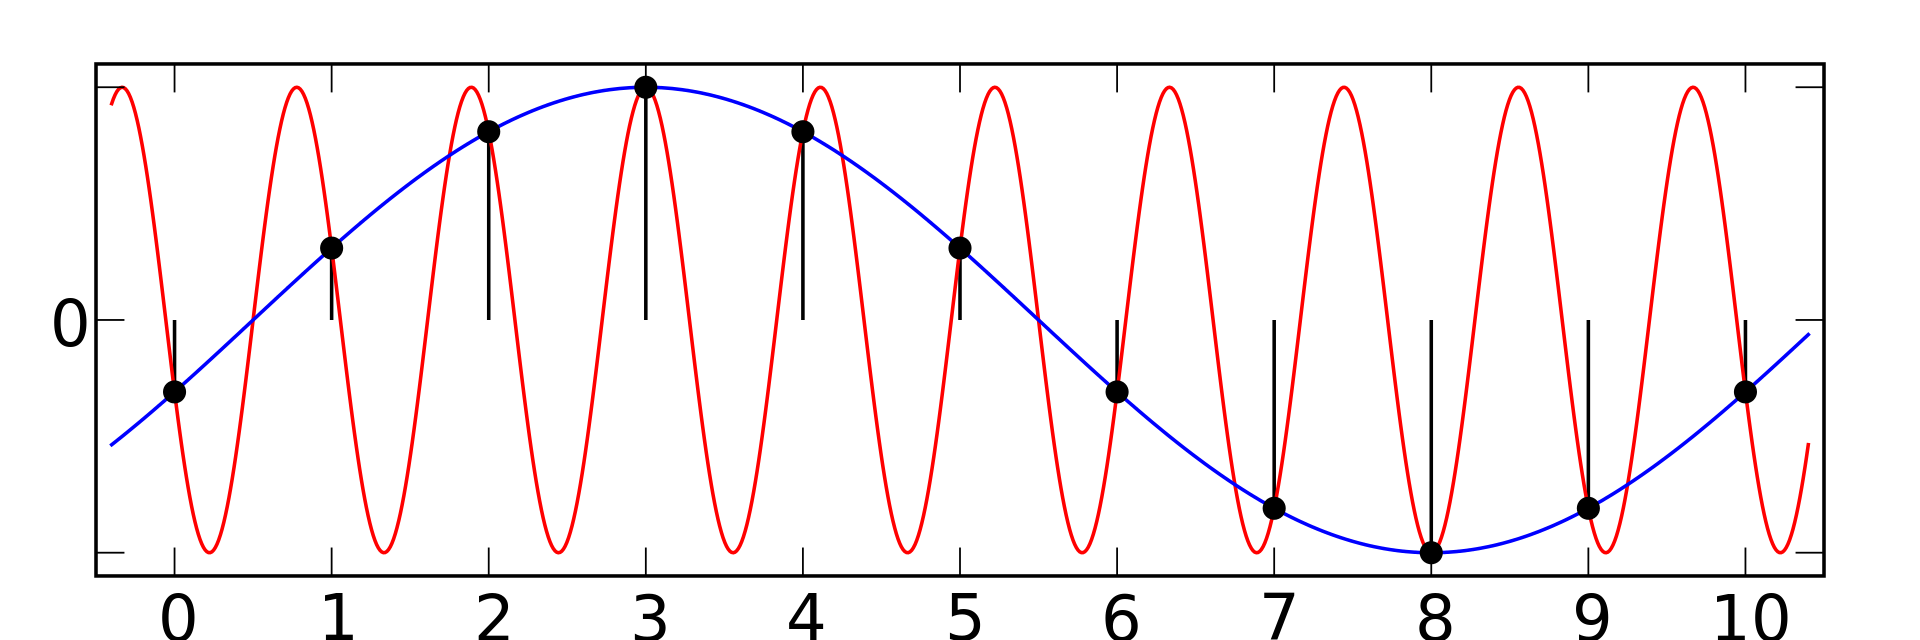
\includegraphics[width=1\textwidth]{Illustrations/AliasingSines.png}
	\caption{Consequences of Aliasing}\cite{ALIASING}
	\label{fig:AliasingSines}
\end{figure}

As seem in Figure \ref{fig:AliasingSines}, if the sampling rate is too small, the signal will 
be aliased and will get a wrong representation of the signal. The red signal represents
the signal to be sampled and obtained, while the blue one is the actual signal obtained, due to a 
smaller than necessary sampling frequency.

\section{Fourier Transform}
As useful as the amplitude might be, for a closer inspection of a signal it is not enough to 
differentiate human speech from different sound sources. Any sound signal can be recreated from 
a combination of sinusoidal signals at different frequencies.  For that reason the Fourier 
Transform can be used to decompose the sound in multiple frequencies. By transforming the 
signal from the time domain to the frequency domain we can get a lot more information about 
a specific signal. By plotting these, we will get the amplitude of each frequency over the whole signal.

\begin{figure}[htp]
	\centering
	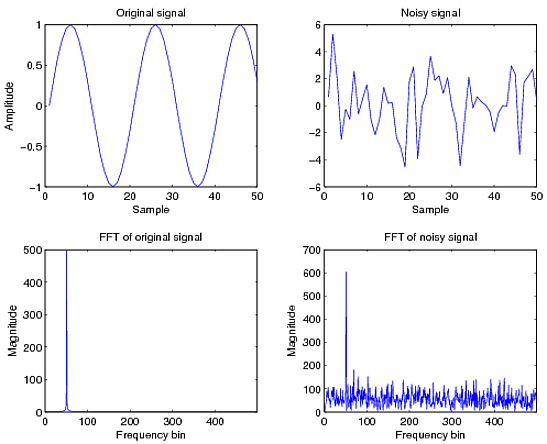
\includegraphics[width=0.6\textwidth]{Illustrations/fftSignals.png}
	\caption{FFT Representation of Two Signals}\cite{FFTPHOTO}
	\label{fig:fftSignal}
\end{figure}
\newpage

As we can see in Figure \ref{fig:fftSignal} besides being able to differentiate between 
different sound sources, especially clean speech, as it was said in a different sections, we 
know the frequencies in which human voice is so we can see it easier in a frequency domain representation, 
we can identify noise easier too.

\section{Spectrogram of a Signal}
Except for perfect examples, just a Fourier transform plot will not be that useful as some
sound sources can be only in a part of the full sample and by viewing the plot over the 
whole sample it will not be accurate enough for filtering. For this reason a spectrogram 
can be used, which instead of taking the Fourier transform over the whole sound sample, it 
will make multiple ones over 0.25 second frames. By doing this we can get 3D plot, where we 
can have the X axis for time or samples, Y axis for the frequencies and color for the amplitude. 
By doing this a really clear representation of the signal can be made from which multiple aspects 
of the signal can be seen and used.
Figures \ref{fig:SpeechSpectrogram} and \ref{fig:NoiseSpectrogram} represent two spectrograms
of speech and noise respectively. The difference can be clearly seen.
\begin{figure}
\centering
\begin{minipage}{.5\textwidth}
	\centering
	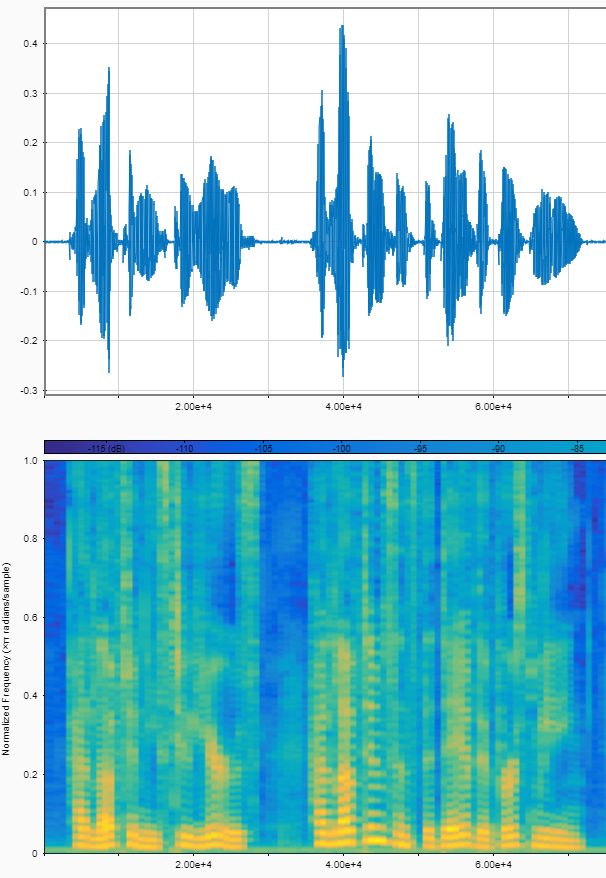
\includegraphics[width=0.6\linewidth]{Illustrations/SpeechSpectrogram.PNG}
	\caption{Speech Spectrogram}
	\label{fig:SpeechSpectrogram}
\end{minipage}%
\begin{minipage}{.5\textwidth}
	\centering
	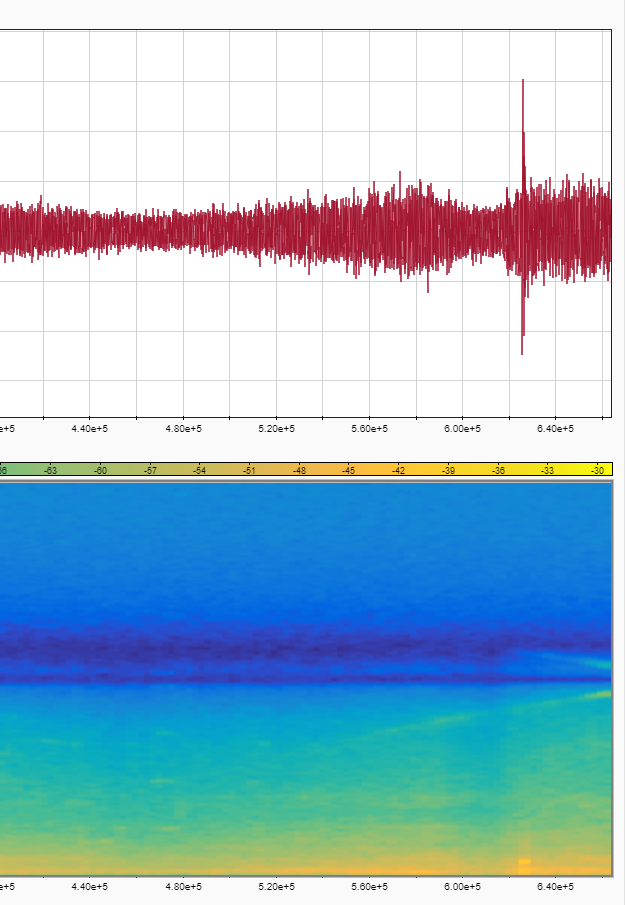
\includegraphics[width=0.6\linewidth]{Illustrations/NoiseSpectrogram.PNG}
	\caption{Noise Spectrogram}
	\label{fig:NoiseSpectrogram}
\end{minipage}
\end{figure}
\newpage
\section{Mel-Frequency Cepstrum}
A Mel-frequency cepstrum is made out of a multitude of Mel-Frequency cepstral coefficients(MFCCs). 
Those are taken from a cepstral representation of the audio sample(or a spectrum of a spectrum).
This can be really useful especially for speech identification as the frequency bands are spaced 
equally on the Mel scale instead of linearly spaced frequency used in a normal cepstrum. 
The mel scale is more useful for this case as it better approximates how humans actually perceive sound.
\cite{MFCC}

\begin{figure}[htp]
	\centering
	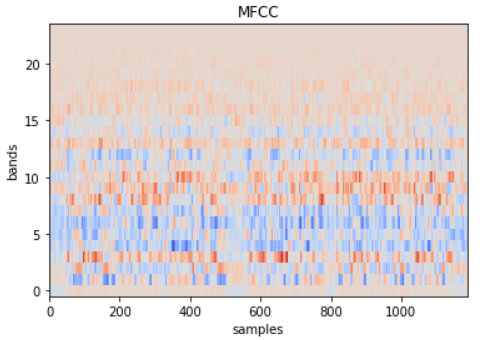
\includegraphics[width = 0.6\textwidth]{Illustrations/mfcc.png}
	\caption{Mel-Frequency Cepstrum Coefficients}
	\label{fig:mfcc}
\end{figure}

\newpage
Besides this, instead of using the full cepstrum, only 24 bands can be used, 
by using the Bark scale instead.
The bark scale is psychoacoustical scale that represents the first 24 critical bands of hearing.
This can easily be made as mel scale and Bark scale are proportional to each other as 1 Bark 
is approximately equal to 100 mels.
By doing this, memory and processing power can be saved by using only 24 bands instead of thousands.
\cite{BARKSCALE}
\begin{figure}[htp]
	\centering
	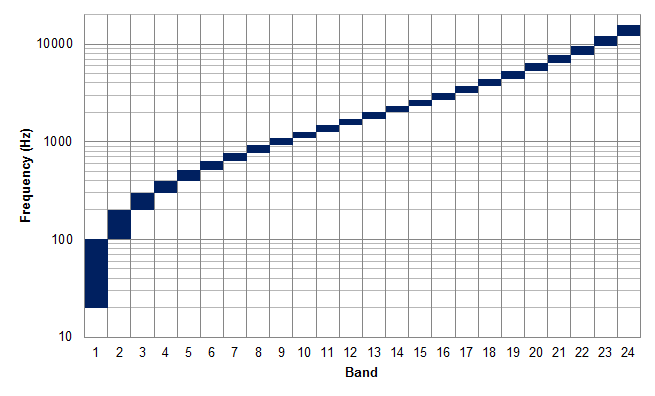
\includegraphics[width=1\textwidth]{Illustrations/Bark_scale.png}
	\caption{The 24 Bands of the Bark Scale}\cite{BARKSCALEPHTOT}
	\label{fig:BarkScale}
\end{figure}

\section{MFCC Sample Modulation}

After the MFCCs were calculated from the sound sample, there isn't really a good way to get the sample back as only 24 band are not enough to get a similar sounding sound sample.
So instead of doing that, the original sample can be modulated using other MFCC values. This,practically will act as a vocoder, as the original signal will be modulated using the spectrum envelope of another.
To do this, the signal will be split in n signal and calculate the discrete fourier transform of each frame, derive the spectrum, and than modulates the spectrum with the coefficients from the MFC and then do inverse DFT to go back to the time domain.